\documentclass[15pt comic sans]{revtex4-2}
%\documentclass[12pt]{article}
\listfiles               %  print all files needed to compile this document

\usepackage{amsmath}
\usepackage{xparse}
\usepackage{graphicx}
\usepackage{dcolumn}
\usepackage{bm}
\usepackage[colorlinks=true,urlcolor=blue,citecolor=blue]{hyperref}
\usepackage{color}
\usepackage{physics}
\usepackage{algorithm2e}
%\usepackage{algorithmic}
\usepackage{algpseudocode}
\usepackage{pgfplots}
\usepackage{pgfplotstable, booktabs, mathpazo}
\usepackage{natbib}

\pgfplotsset{compat=1.15}

\pgfplotstableset{
    every head row/.style={before row=\toprule \hline ,after row=\hline\hline \midrule},
    every last row/.style={after row=\hline \bottomrule},
    every first column/.style={
        column type/.add={|}{}
        },
    every last column/.style={
        column type/.add={}{|}
        },
}
\pgfplotstableset{
    every head row/.style={before row=\toprule \hline ,after row=\hline\hline \midrule},
    every last row/.style={after row=\hline \bottomrule}
}

%\begin{figure}[hbtp]
%\includegraphics[scale=0.4]{.pdf}
%\caption{}
%\label{fig:}
%\end{figure}

%\begin{tikzpicture}
%    \begin{axis}[
%            title= Earth-Sun system, Forward Euler integration,
%            xlabel={$x$},
%            ylabel={$y$},
%        ]
%        \addplot table {../runresults/earthEuler2body.dat}
%    \end{axis}
%\end{tikzpicture}

\begin{document}
\title{%
	project 1, FYS-STK4155 \\
	\large Regression and Resampling of Terrain data and the Franke function}
\author{A. G. Eriksen}
\date{\today}
\begin{abstract}
	Exploration of machine learning methods by the Regression subfamily.
	The methods were tested on a simulated surface generated by the Franke-function.
	Initially, regressed with Ordinary least squares regression before
	expanding to Ridge. Exploration of resampling methods also performed, with
	bootstrap and k-fold CV. Intent was to also implement the LASSO regression method
	and introduce real data to the models. This fell through.
\end{abstract}
\maketitle
\tableofcontents

\section{introduction}
%The aims and rationales of the project. What we have done in the project. Brief 
%summary of structure of the report. 

The motivation for this project was in large part to explore regression methods as a
subset of machine learning. Machine learning bases itself mainly on a frequentist approach,
or frequency or proportion of data as a metric for prediction. The regression methods have
a relatively intuitive setup and serves as a good entry point for exploring machine learning
as well as being usefull for predicting numerical problems suspected of following an unknown
function.\\
Three methods were decided on to explore, ordinary least squares(OLS), Ridge regression and
Lasso regression. OLS was performed with results approximating the expectations for regressions
of our dataset. Ridge was barely runnable, but lacked any finish w.r.t. storing and displaying the
data from it. Lasso regression fell off completely.\\
Beyond the regressor models, we also utilized resampling methods, Bootstrap and k-fold Cross Validation.
These methods allow us to make the best use out of the data already in our possession, as the resampling
helps average over several smaller "data sets" sampled from a majority of the initial data. The results
from these smaller sets are compared to the minority of the original which has been left untouched. The
amount of tests allows us to control for e.g. variance and bias.\\
Once these methods were laid out and tested, the idea was to move on to real data, rather than the simulation
and make use of terrain data from Norway. Due to time constraints, this did not happen.\\
The report here is structured into a method section where I generally go through the assumptions, models and
algorithms for the methods mentioned. Following this, is a section of the few results I managed to collect
and an attempt at discussing them as they relate. Finally, the conclusion attempts to conclude what can be
from concluded after the run. Also here, I attempt to describe the issues with the implementation as well
as the state of the project and how they might be improved.

\section{method}
%Theoretical models and technicalities
The initial assumption we make in regression is that our data set and targets are connected with
some function. Thus, we can write 
\begin{align}
	\bm{y} = f(\bm{x}) + \varepsilon.
\end{align}
Here, $y$ is the targets we wish to predict and the $x$ are our input variables. The $\varepsilon$ 
represents an unknown noise in the function. Given this function, we want to approximate the targets
using some model. Therefore, we set
\begin{align}
	\bm{\tilde{y}} = \bm{X}\bm{\beta},
\end{align}
which approximates $f(\bm{x})$. Since we want to predict the targets, we need some measurement of
how well we fit the model. This comes in the form of a cost function which we can minimize to find 
the optimal fit. 
\begin{align}
	C(\bm{\beta}) &= \frac{1}{n} \big\{ ( \bm{y} - \bm{X}\bm{\beta} )^2 \big\} ,
	\label{costfunc}\\
	\pdv{C(\bm{\beta}}{\bm{\beta}} &= 0 = \bm{X^T}\qty(\bm{y} - \bm{X}\bm{\beta}), \\
	\bm{\hat{\beta}} &= \qty(\bm{X^T}\bm{X})^{-1} \bm{X^T}\bm{y}.
	 \label{betaoptimal}
\end{align}
$\hat{\beta}$ is the optimal coefficients for the model.\cite{hastie2009elements} \cite{morten2020lecturenotes} \\


With an expression for $\beta$ ready, we need a system to fit to. This comes in the way of
Franke's function\cite{franke1979critical}
\begin{align}
 f(x,y) &= \frac{3}{4}\exp{\left(-\frac{(9x-2)^2}{4} - \frac{(9y-2)^2}{4}\right)} 
	\nonumber\\
		&+\frac{3}{4}\exp{\left(-\frac{(9x+1)^2}{49}- \frac{(9y+1)}{10}\right)} 
	\nonumber\\
		&+\frac{1}{2}\exp{\left(-\frac{(9x-7)^2}{4} - \frac{(9y-3)^2}{4}\right)} 
	\nonumber\\
		&-\frac{1}{5}\exp{\left(-(9x-4)^2 - (9y-7)^2\right) }.
\label{franke}
\end{align}
This function, we define over an area $x, y \in [0, 1]$. In addition, noise can be added to the 
function to obscure the functional relationship between the points in the function.

This system then consists of the input data, $x,y$ and the output data $z$. Having generated
the inputs and found the target, the next step is to split the data into training and test sets
and define a feature matrix as a model for the system. 

As we have settled on regression methods, we have chosen to fit $z$ with a polynomial model, where
the model complexity would represent the degree of polynomial used to set up the model. In our
case the inputs amount to 2 vectors, so the algorithm for making the feature matrix becomes 
as in algorithm \ref{alg:design}

\begin{algorithm}
	\DontPrintSemicolon
	\KwIn{$\bm{x}$ and $\bm{y}$ and polynomial degree $n$}
	\KwOut{Feature matrix X with dimension $mxn$}
	$n \gets length(\bm{x})$\;
	$m \gets int((n+1)\cdot (n+2)/2)$\;
	$X \gets matrix.ones(nxm)$\;
	\For{$i \gets 1$ \textbf{to} $n+1$}{
		$q \gets int((i)*(i+1)/2)$\;	
		\For{$k \gets 0$ \textbf{to} $i+1$}{
			$X_{(:, q+k)} \gets x^{i-k}\cdot y^k$\;
		}
	}
	\Return{$X$}\;
\caption{make feature matrix X given input $\vec{x}, \vec{y}$ and dimension n}
\label{alg:design}
\end{algorithm}

With an algorithm for the feature matrix and a set of targets generated by the Franke 
function we just need to fit the features and predict an output. Following this, we can 
apply various statistics to compare the model to the targets. These would include
\begin{align}
	MSE(y, \tilde{y}) &= \frac{1}{n}\sum_{i=0}^{n-1}(y_i - \tilde{y_i})^2
		= \mathbb{E}[(y - \tilde{y})^2],
		\label{MSE} \\
	R^2(y, \tilde{y}) &= 1 - \frac{\sum_{i=0}^{n-1}(y_i - \tilde{y_i})^2}
		{\sum_{i=0}^{n-1}(y_i - \mathbb{E}[y])^2} 
		\label{R2}, \\
	\mathbb{E}[y] &= \frac{1}{n}\sum_{i=0}^{n-1} y_i \label{mean}, \\
	\mathbb{E}[(y - \tilde{y})^2] 
		&=...= \mathbb{E}[(y -\mathbb{E}[\tilde{y}])^2] 
			+ \mathbb{E}[(\tilde{y} - \mathbb{E}[\tilde{y}])^2] 
			+ \sigma^2 \label{bias-variance-error}, \\
	\mathbf{Bias}(y, \tilde{y} &= \mathbb{E}[(y -\mathbb{E}[\tilde{y}])^2] ,
		\label{bias} \\
	\mathbf{Var}(\tilde{y}) &= \mathbb{E}[(\tilde{y} - \mathbb{E}[\tilde{y}])^2] ,
		\label{variance} \\
	MSE(y, \tilde{y}) &= \mathbf{Bias}(y, \tilde{y}) + \mathbf{Var}(\tilde{y}) + \sigma^2
		\label{bias-variance}.
\end{align}

Moving on from this, we can begin to refine the data we have somewhat, using resampling 
methods. The ones we will make use of, are Bootstrap and k-fold Cross Validation. 
The essence here, is that we have a limited data set. To compensate for this, methods of
selecting which data to run allows us to make the best use of what data we do have. 
The main methods discussed here are Bootstrap[\ref{alg:bootstrap}] and k-fold Cross 
Validation[\ref{alg:kfoldCV}]

\begin{algorithm}
	\DontPrintSemicolon
	\KwIn{feature matrix, $X$, targets, $y$, and number of bootstraps, $N$}
	\KwOut{model fits and predictions}
	$\bm{\tilde{y}^{fit}} \gets \mathbf{array}(N)$\;
	$\bm{\tilde{y}^{predict}} \gets \mathbf{array}(N)$\;
	$\bm{\beta} \gets \mathbf{array}(N)$\;
	\For{$i \gets 0$ \textbf{to} $N$}{
		Shuffle $X$ and $y$\;
		Split data into training and test sets\;
		$\beta \gets OLS(X_{train}, y_{train})$\;
		$\tilde{y}_i^{fit} \gets \bm{X_{train}}\bm{\beta}$\;
		$\tilde{y}_i^{predict} \gets \bm{X_{test}}\bm{\beta}$\;
	}
	\Return{$\bm{\beta}$, $\bm{\tilde{y}_{fit}}$, $\bm{\tilde{y}_{predict}}$}
	\caption{The Bootstrap method of resampling. This method makes no distinction
	between resamplings, using the assumption that the initial set follows a 
	distribution the resampling is mimicing. Thus, the values approaches a better 
	interpretation}
	\label{alg:bootstrap}
\end{algorithm}

\begin{algorithm}
	\DontPrintSemicolon
	\KwIn{feature matrix, $\bm{X}$, targets, $\bm{y}$, and number of folds, $k$}
	\KwOut{model fits and predictions}
	$\tilde{y}^{fit} \gets \mathbf{array}(k)$\;
	$\tilde{y}^{predict} \gets \mathbf{array}(k)$\;
	$\bm{\beta} \gets \mathbf{array}(k)$\;
	Split $k$ folds $\bm{\mu}, \bm{\nu} \subset \bm{X}, \bm{y}$\;
	\For{$i \gets 0$ \textbf{to} $k$}{
		$\bm{X^{test}} \gets \bm{X}\{\mu_i\}$\;
		$\bm{X^{train}} \gets \bm{X}\{\bm{\mu} - \mu_i\}$\;
		$\bm{y^{test}} \gets \bm{y}\{\nu_i\}$\;
		$\bm{y^{train}} \gets \bm{y}\{\bm{\nu} - \nu_i\}$\;
		$\beta \gets OLS(X_{train}, y_{train})$\;
		$\tilde{y}_i^{fit} \gets \bm{X_{train}}\bm{\beta}$\;
		$\tilde{y}_i^{predict} \gets \bm{X_{test}}\bm{\beta}$\;
	}
	\Return{$\bm{beta}$, $\bm{\tilde{y}^{fit}}$, $\bm{\tilde{y}^{predict}}$}
	\caption{k-fold Cross Validation method of resampling. This allows us to vary the 
	combination of the shuffled indices without reusing datapoints.}
	\label{alg:kfoldCV}
\end{algorithm}

Finally, we can also look more closely at the regression method we use. The Ordinary 
Least Squares solution works OK, but there are issues, for instance if $(X^TX)^{-1}$
were to be singular, then the method would fail. A solution to this lies in methods
such as Ridge regression and Lasso regression. The solution to the possibility of 
the singular values lies in adding something along the diagonal, so
$(X^TX + \lambda\mathbb{I})^{-1}$\\

This complicates the expression for MSE somewhat, due to this addition. A rewrite of the 
MSE, could be made using the "norm-2" description to
\begin{align}
	\min_{\beta\in\mathbb{R}^p} =
		\frac{1}{n} \sum_{i=0}^{n-1} (y_i - \tilde{y}_i)^2 
		\frac{1}{n} \norm{\bm{y} - \bm{X\beta}}_2^2.
\end{align}
If we were to add our extra parameter here, we could 
\begin{align}
	\min_{\beta\in\mathbb{R}^p}\qq{} \frac{1}{n}\norm{\bm{y} - \bm{X\beta}}_2^2 
		+	\lambda\norm{\bm{\beta}}_2^2
\end{align}
Which gives us what we call Ridge regression, or we could use "norm-1" to set
\begin{align}
	\min_{\beta\in\mathbb{R}^p}\qq{} \frac{1}{n}\norm{\bm{y} - \bm{X\beta}}_2^2 
		+	\lambda\norm{\bm{\beta}}_1.
\end{align}
Each of these represent various ways to ensure we get a minimum. The effects differ 
somewhat between them, where Ridge "penalizes" some betas according to the amount of
variance in the system, Lasso strikes these out, setting them to 0, while keeping the 
unaffected $\beta$'s essentially the same. \\

The code is set up so that a mesh of 2 matrices are fed into the franke function and
then all three are flattened into 1 dimension. Then they are fed into a resampling and
regression function where the above mentioned mathematics takes place and after this, 
the resulting fit and predictions for the target values are subjected to various error
tests, such as MSE, R2 score and bias-variance estimations

With regards to the bias-variance estimations and their relationship to the error 
estimate can be expressed

\begin{align}
    & C(\mathbf{\hat{X}}, \vec{\beta}) 
		 = \frac{1}{n} \sum_{i=0}^{n-1}(y_i - \tilde{y}_i)^2
		 \,=\, \mathbb{E}[(y- \tilde{y})^2]
\end{align}
using the values for: $y = f(x) + \varepsilon$, $f(x) \equiv f$, 
$\ev{\varepsilon} \equiv 0$ and $var(\varepsilon)\equiv \sigma^2$, as well as adding and
subtracting $\mathbb{E}[\bm{\tilde{y}}]$
\begin{align}
	\mathbb{E}[(y- \tilde{y})^2] 
	&	= \mathbb{E}[(y - \tilde{y} + \mathbb{E}[\bm{\tilde{\tilde{y}}}] 
		- \mathbb{E}[\bm{\tilde{y}}])^2] \nonumber \\
	&= \mathbb{E}[(f-\ev{\tilde{y}})^2] 
	+ \mathbb{E}[(\tilde{y} - \ev{\tilde{y}})^2] 
	+ \mathbb{E}[\varepsilon^2] \nonumber\\
	&+ 2\mathbb{E}[(f-\mathbb{E}[\bm{\tilde{y}}])(\bm{\tilde{y}} 
		- \mathbb{E}[\bm{\tilde{y}}])] \nonumber\\
	&+ 2\mathbb{E}[\varepsilon(f-\ev{\tilde{y}})] 
	+ 2\mathbb{E}[\varepsilon(\bm{\tilde{y}} - \mathbb{E}[\tilde{y}])]
\end{align}
Here we have 2 parts with the expectation value of our noise variable, which can be 
separated out ab both $\bm{f}$, $\bm{\tilde{y}}$ and $\bm{\tilde{y}}$ are assumed
deterministic. Since the noise has a mean value of $0$, these parts dissapear. 
Additionally, $\mathbb{E}[\varepsilon]=\sigma^2$.
\begin{align}
	= \mathbb{E}[(f-\ev{\tilde{y}})^2] 
	+ \mathbb{E}[(\tilde{y} - \ev{\tilde{y}})^2] 
	+ \mathbb{E}[\varepsilon^2]
	+ 2\mathbb{E}[(f-\mathbb{E}[\bm{\tilde{y}}])
\end{align}
Next bit requires a little bit of work, but 
Wolframalpha\cite{wolframalpha2020expval} lets us set 
$\mathbb{E}[f\cdot\bm{\tilde{y}}]$, which we can separate as they're both deterministic
so, $ \mathbb{E}[f]\mathbb{E}[\bm{\tilde{y}}] - \mathbb{E}[\bm{\tilde{y}}]^2 $, which
cancels out, seeing as both the function and the approximation share an expected value
given the initial assumption of the model. This leaves us with 
\begin{align}
	\mathbb{E}[(y- \tilde{y})^2] 
	= \mathbb{E}[(f-\ev{\tilde{y}})^2] 
	+ \mathbb{E}[(\tilde{y} - \ev{\tilde{y}})^2] 
	+ \mathbb{E}[\varepsilon^2]
     = Bias[\tilde{y}] + Var[\tilde{y}] - \sigma^2.
\end{align}
The bias, variance and noise variance is in order here. The bias represents an offset
between the model mean and the target values, the variance is a measure of the spread of
the models with regards to the mean of all the models, while the noise variance is 
generally unknown and harder to pin down. 

\section{results}
%Results of study and discussion of results

In essence, these regressions are performed to make a model of and predict the shape of
(simulated) terrain. While most of the simulations here have been performed with a
much more significant level of noise added on to the base function, the surface shown
can be seen in figure \ref{fig:FrankeSurface}

\begin{figure}[hbtp]
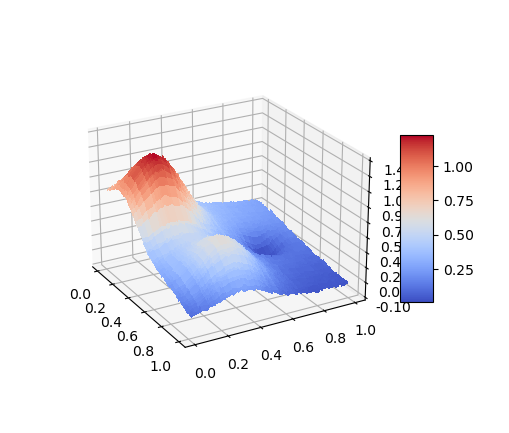
\includegraphics[scale=0.7]{../plots/surfaceplotfrankeSigma01.png}
\caption{Surface plot of the simulated surface generated through the Franke function
	The inputs and outputs are both unitless, so the axes are merely ilustrative. 
	This figure was generated using a slight amount of noise added to the function, 
	which is the source of the slight irregularities observed. The variance of the 
	noise was set to $0.01$ for the sake of illustrating the surface, while most of the 
	results taken from the function uses a variance of 1, which makes the structures 
	seen here obscured.}
\label{fig:FrankeSurface}
\end{figure}

For the most basic implementation of regression, with no regard for the possibility of a
singular matrix and with the assumption of a large enough data set that the prediction 
is accurate. Here, we set up the data and prepare several different models, based on the
degree of the polynomial we want to use to make our fit. To visualise the accuracy of 
the fit, a plot of the MSE for the fit to the training data and the test data are set up.


\begin{figure}[hbtp]
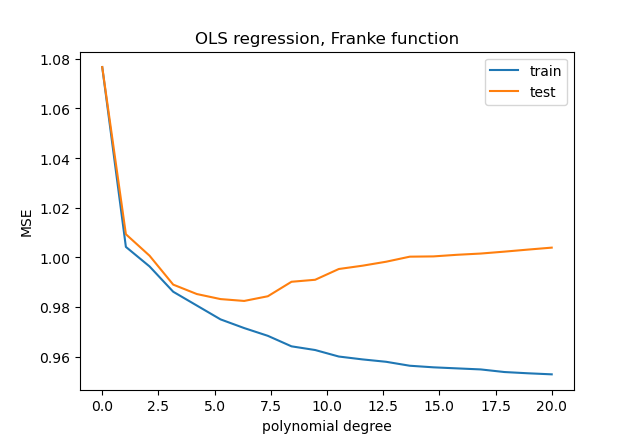
\includegraphics[scale=0.7]{../plots/frankeOLSMSEsigma1maxdeg20.png}
\caption{Plot of the MSE for OLS regression of the Franke function with no resampling
	techniques active. The worst fit is for the straight line case, where the MSE lies
	at about a 1, with a rapid reduction which smooths out around 5th degree polynomial
	for the test set, while the training fit continues to improve. 
	Couple of notices here, is the floating point numbers that represent the model 
	complexity or polynomial degree. They should be integers. In addition, there was 
	no real fit for the 0th degree polynomial, and the starting point here is not 
	accurate}
\label{fig:MseNoResample}
\end{figure}

Following after these, there was the issue of implementing resampling methods. Since 
these also give us several fits of the model, we can also evaluate the variance of the
models across tries to produce a bias-variance plot,

\begin{figure}[hbtp]
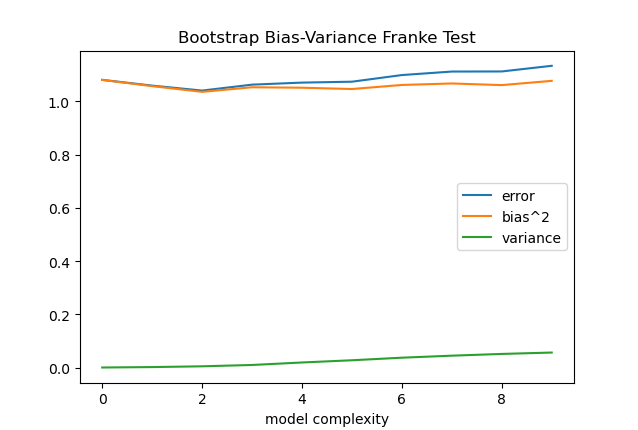
\includegraphics[scale=0.7]{
	../plots/frankeBootstrapBiasVariancesigma1poly10boot1e3datapt1e6test.png}
\caption{
	Here we have the bias and variance plot of a run with bootstrap, running $1e3$ 
	resamplings over $1e6$ data points with a noise strength of $1$ and fitting to the training
	set. We see that the bias starts out very high and gradually increases. The variance begins 
	very small, and then slowly increases. The summed up error roughly follows the 2, but there 
	is a distinct difference in the behaviour for the error here and in figure 
	\ref{fig:MseNoResample} with regards to the error's behaviour over the model's increasing 
	complexity. 
	}
\label{fig:BootstrapBiasVariance1e6test}
\end{figure}
Figure \ref{fig:BootstrapBiasVariance1e6test} shows a high and increasing bias and a slowly
growing variance over the model complexity kept the same as in figure 
\ref{fig:MseNoResample}.

This is largely the extent of gathered data. Further examples of the bias variance 
results should be in the appendix. 

\section{conclusion}
%Beyond discussion, this is actually concluding things. 
%perspectives of study

The setup of the Franke function as well as the surface plot of the generated data was 
largely taken from the project description and looks about as you'd expect. The example 
with no resampling and Ordinary least squares also behaves as we would expect, where the 
initial bias of the linear fit drops off as we introduce complexity until the point 
where the variance's exponential growth overtakes the dropping bias and we see the test 
error increase. \\

For some reason, this seems to not be the case when the Bootstrap method is introduced, 
as we see in figure \ref{fig:BootstrapBiasVariance1e6test}.  Here, the bias doesn't fall off 
for some reason and the variance hardly increases at all compared to the increase in 
error we saw when looking at the simplest case. This could be an error in the calculation
of the new measurements, with the number of fits per model degre of complexity increases. 
Perhaps it's an error regarding the dimensionality along which we took the means for the
difference in the bias and variance. Mixing up the rows and collumns as it were. \\

That said, there were several things wrong in the code, and while I eventually managed to 
finish a calculation using the k-fold cross validation, the amount or repeated code showed
it's toll in strange errors. Though the code was attempted cleaned up and object oriented 
in order to reduce copying code and making the usecase more general, especially wrt.
including the real terrain data. These attempts did not bear fruit, unfortunately, as when
I finally managed to get a working example of the simplest case, the results were strange, 
even just the measure of the MSE. 

Another issue I encountered was difficulties in selecting which data to keep. The 
$\bm{\beta}$ coefficients would definitely be a good idea. Perhaps also the train and
test indices, as well as the training and test fits of the model. I did not settle on a 
method I was happy with. Further usefull data, not the least in the case of plots were the
MSE, bias, etc. which would need to be stored or used for each iteration of each of the 
varying parameters. 

I'd think the main improvement for this project would be a more carefully setup, object
oriented design so that the varying resampling and regression methods would be more 
easily changed without retyping so many initial variables and data, as these quickly 
accumulated errors and made the code very tiresome to navigate. Further, this would 
make entering in the actual terrain data much easier and would help guarantee the results
could be comparable between the to usecases given no changes were made to the code running
on the data sets.

\section{appendix}
%extra material, e.g. superfluous code, tables and figures not fitting into the text itself.


\begin{figure}[hbtp]
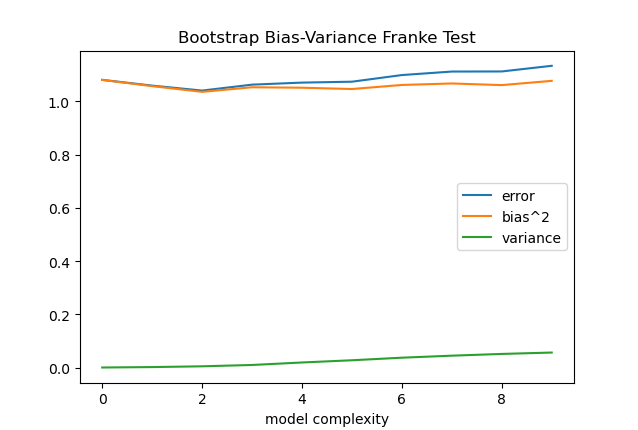
\includegraphics[scale=0.7]{
	../plots/frankeBootstrapBiasVariancesigma1poly10boot1e3datapt1e4test.png}
\caption{
	Bias, variance and error for the bootstrap resampling of the franke data fitted to 
	the test set. $1e3$ bootstraps and $1e4$ data points input. 
	}
\label{fig:BootstrapBiasVariance1e4test}
\end{figure}

\begin{figure}[hbtp]
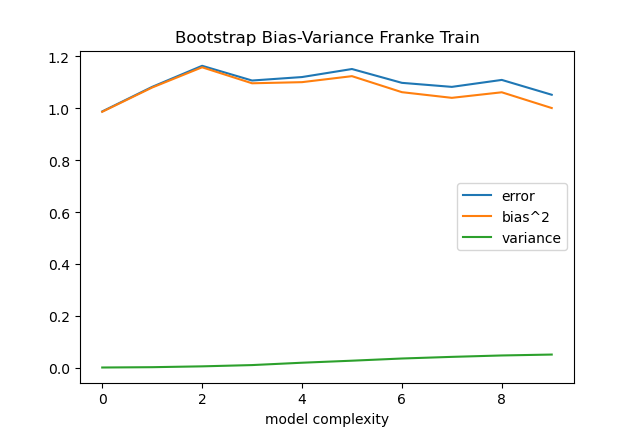
\includegraphics[scale=0.7]{
	../plots/frankeBootstrapBiasVariancesigma1poly10boot1e3datapt1e4train.png}
\caption{
	Bias, variance and error for the bootstrap resampling of the franke data fitted to 
	the train set. $1e3$ bootstraps and $1e4$ data points input. 
	}
\label{fig:BootstrapBiasVariance1e4train}
\end{figure}

\begin{figure}[hbtp]
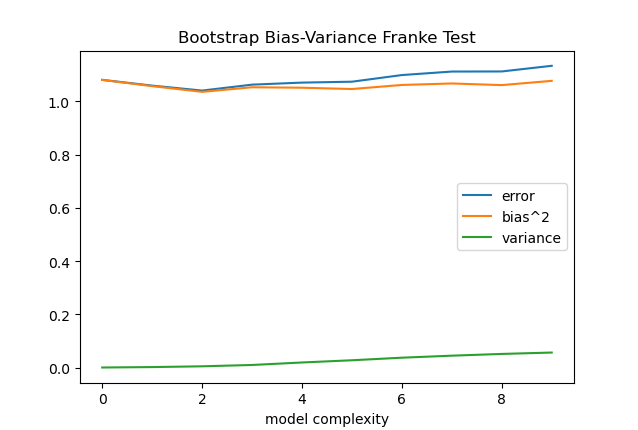
\includegraphics[scale=0.7]{
	../plots/frankeBootstrapBiasVariancesigma1poly10boot1e3datapt2e4test.png}
\caption{
	Bias, variance and error for the bootstrap resampling of the franke data fitted to 
	the test set. $1e3$ bootstraps and $2e4$ data points input. 
	}
\label{fig:BootstrapBiasVariance2e4test}
\end{figure}

\begin{figure}[hbtp]
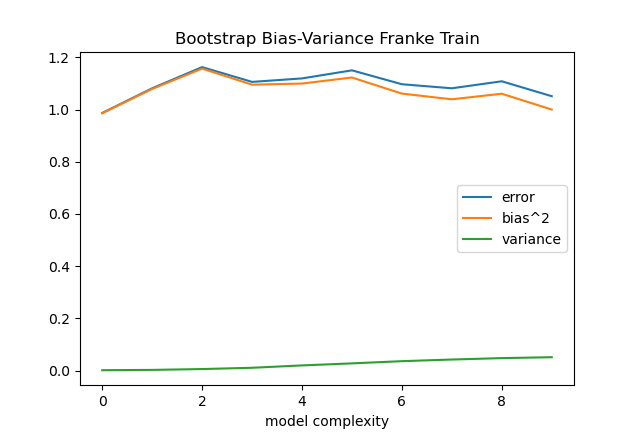
\includegraphics[scale=0.7]{
	../plots/frankeBootstrapBiasVariancesigma1poly10boot1e3datapt2e4train.png}
\caption{
	Bias, variance and error for the bootstrap resampling of the franke data fitted to 
	the train set. $1e3$ bootstraps and $2e4$ data points input. 
	}
\label{fig:BootstrapBiasVariance2e4train}
\end{figure}

\begin{figure}[hbtp]
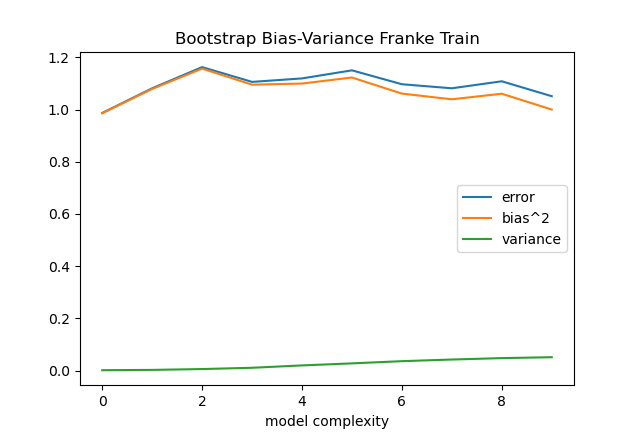
\includegraphics[scale=0.7]{
	../plots/frankeBootstrapBiasVariancesigma1poly10boot1e3datapt1e6train.png}
\caption{
	Bias, variance and error for the bootstrap resampling of the franke data fitted to 
	the train set. $1e3$ bootstraps and $1e6$ data points input. 
	}
\label{fig:BootstrapBiasVariance1e6train}
\end{figure}

\bibliography{bib.bib}
\end{document}

